\documentclass[a4paper,10pt,twoside,twocolumn]{dndbook} %a4, 10pt, book (idk why i did that...), 2 cols, dnd-themed
\usepackage[english]{babel} %language
\usepackage[utf8]{inputenc} %lovely utf-8
\usepackage{graphicx} %images
\usepackage{wrapfig} %images
\usepackage{array} %allways use this shit, idk why
\usepackage{tikz} %draw stuff
\usepackage{ifthen} %draw stuff
\usetikzlibrary{shapes,calc,fadings} %draw stuff
\usepackage{xspace} %usefull idk, allways import this stuff
\usepackage{dirtytalk} %\say because fuck it
\usepackage{setspace} %don't ask, kind of like it...
\usepackage{pgfplots}

\usepackage[singlelinecheck=false]{caption} %idk dndbook...
\usepackage{listings} %idk dndbook...
\usepackage{shortvrb} %not used yet...
\usepackage{stfloats} %idk dndbook
\usepackage{dirtytalk}

\singlespacing
\makeatletter %because of titlepage and \HUGE

\@openrightfalse %no empty pages

\graphicspath{ {./images/} }

\def \license {GNU Free Documentation License}
\def \licensetext {Please consider and respect the copyleft of this license. The content of this document should be accessible to everyone. Everyone has the right to use the content of this document as he/she wishes, to modify it, to publish it modified (taking into account the copyleft) and to republish it without any changes (taking into account the copyleft).}
\def \author {Sven Hugi}%if you edit this document, add your name... <3
\def \illustrators {} %add name
\def \othercontrib {} %add name

%highlighting with some random effect -> looks handmade and i love it...
\newcommand\hl[2][yellow]{
	\begin{tikzpicture}[
	baseline,
	decoration={random steps,amplitude=1pt,segment length=15pt},
	outer sep=-15pt, inner sep = 0pt
	]
	\node[decorate,rectangle,fill=#1,anchor=text]{#2\xspace};
	\end{tikzpicture}
}
%2 column layout hack...
\newcommand{\nextPage}{
	\newpage
	\hbox{}
	\newpage
}
%make bad things look ok...
\newcommand{\doublelinebreak}{
	\linebreak\linebreak
}
%the old HUGE fontsize
\newcommand\HUGE{\@setfontsize\Huge{60}{80}} 

\renewcommand{\maketitle}{
	\thispagestyle{empty}
	\onecolumn %fuck it
	\vspace*{5cm}
	\begin{center}
		$\vspace*{2cm}$
			{\HUGE\DndFontDropCap{LEMMY}}\\	
	\end{center}
	\twocolumn %reset shit
}\makeatother

\begin{document}
	\maketitle
	\section*{Credits}
	\vspace{.25cm}
	\textbf{Authors:} \author\linebreak
	\textbf{Illustrators:} \illustrators\linebreak
	\textbf{Additional Contributors:} \othercontrib\linebreak
	\textbf{License:} \license\doublelinebreak
	\licensetext\doublelinebreak
	The image is from Wikipedia -.-
	\vfill\pagebreak\hbox{}\vfill\hfill{\tiny This Document was written in \LaTeX.}
	\tableofcontents
	%\chapter{Lemmy}
	\begin{center}
		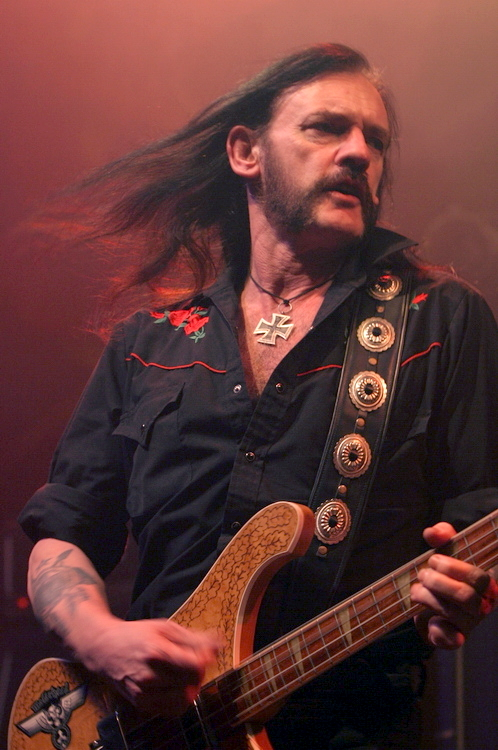
\includegraphics[width=\linewidth]{Lemmy.jpg}
	\end{center}
	
	\say{I don't do regrets. Regrets are pointless. It's too late for regrets. You've already done it, haven't you? You've lived your life. No point wishing you could change it.}
	\begin{flushright}
		\noindent\rule{8cm}{0.2pt}\\
		\begin{spacing}{0.75}
			\textit{Lemmy}
		\end{spacing}
	\end{flushright}
	\vspace{0.5cm}
	\say{Don't look to me. Don't ask for help. Don't ask for anything that you can do yourself.}
	\begin{flushright}
		\noindent\rule{8cm}{0.2pt}\\
		\begin{spacing}{0.75}
			\textit{Lemmy}
		\end{spacing}
	\end{flushright}
	\vspace{0.5cm}
	\say{It seems that our brave new world is becoming less tolerant, spiritual and educated than it ever was when I was young.}
	\begin{flushright}
		\noindent\rule{8cm}{0.2pt}\\
		\begin{spacing}{0.75}
			\textit{Lemmy}
		\end{spacing}
	\end{flushright}
	\vspace{0.5cm}
	\say{In your twenties, you think you are immortal. In your thirties, you hope you are immortal.}
	\begin{flushright}
		\noindent\rule{8cm}{0.2pt}\\
		\begin{spacing}{0.75}
			\textit{Lemmy}
		\end{spacing}
	\end{flushright}
	\vspace{0.5cm}
	\section{Extended Spell List}
	\begin{DndTable}[header=Spell List]{lX}
		\textbf{Spell Level}	&\textbf{Spells}\\
		$1st$					&Guiding Bolt, Mage Armor\\
		$2nd$					&Heat Metal, Zone of Truth\\
		$3rd$					&Beacon of Hope, Fireball\\
		$4th$					&Stoneskin, Wall of Fire\\
		$5th$					&Skill Empowerment, Flame Strike\\
	\end{DndTable}
	\section{Level 1}
	\subsection{Don't ask for Help}
	Your hit-dice is increased to a d10.
	\subsection{Rock 'n Roll}
	You gain proficiency with a instrument of your choice.
	\subsection{Song of Rest}
	Beginning at 1st level, you can use soothing music or oration to help revitalize your wounded allies during a short rest. If you or any friendly creatures who can hear your performance regain hit points at the end of the short rest by spending one or more Hit Dice, each of those creatures regains an extra 1d6 hit points.
	\section{Level 6}
	\subsection{I don't do regrets}
	Beginning at 6th level, you can attack twice, instead of once, whenever you take the Attack action on your turn. The number of attacks increases to three when you reach 14th level in this subclass.
	\subsection{Lemmy, I need a Beer}
	You can always ask Lemmy if you could get a beer.
	\section{Level 10}
	\subsection{educated}
	You can add your intelligence modifier to charisma checks.
	\section{level 14}
	\subsection{Let's Fight}
	You gain proficiency with martial melee weapons.
\end{document}